\title{Error Analysis in PHYS180}
\author{Jordan C. Hanson}
\date{\today}
\documentclass[12pt]{article}
\usepackage[margin=2cm]{geometry}
\usepackage{amsmath,mathtools}
\usepackage{graphicx}

\begin{document}
\maketitle

\begin{abstract}
Scientific measurements cannot be quoted without an assessment of the precision.  We quantify this precision in the form of error analysis.  Rather than originating from \textit{human error}, \textit{statistical errors} arrise from the intrinsic uncertainty encounted in measuring quantities with real instruments.  Further, errors \textit{propagate} through calculations.
\end{abstract}

\section{Instrumental Precision}

The instrumental precision of a piece of data is determined by the smallest division on the instrument.  For example, suppose a length is measured with a meter stick, and the smallest divisions on the meter stick are 1 millimeter.  If the length measured is 31.0 cm, then that result must be stated as $31.0\pm0.1$ cm.

\section{Accuracy versus Precision}

Accuracy and precision are not the same concept.  Accuracy is how far the measured result is from the true value, whereas precision compares the statistical error of a measurement to the measured value itself.  A measurement of $31.0\pm0.1$ cm is precise, because 0.1 cm is small compared to 31.0 cm.  It is not \textit{accurate} if the true length is 29.0 cm.  Why? Because the numbers 31.0 cm and 29.0 cm are separated by $(31.0-29.0)/0.1 = 20$ factors of the error.

\section{Statistical or Random Error}

Suppose a measurement is made with a dial, where a needle is pointing to a number, but vibrating.  When the dial is read one moment, it reads $101.3$ kPa, and in another moment, $101.2$ kPa.  Which pressure measurement of the atmosphere is correct?  It turns out that upon repeated measurements, the \textit{distribution} of measurements resembles Fig. \ref{fig:histo}.

\begin{figure}
\centering
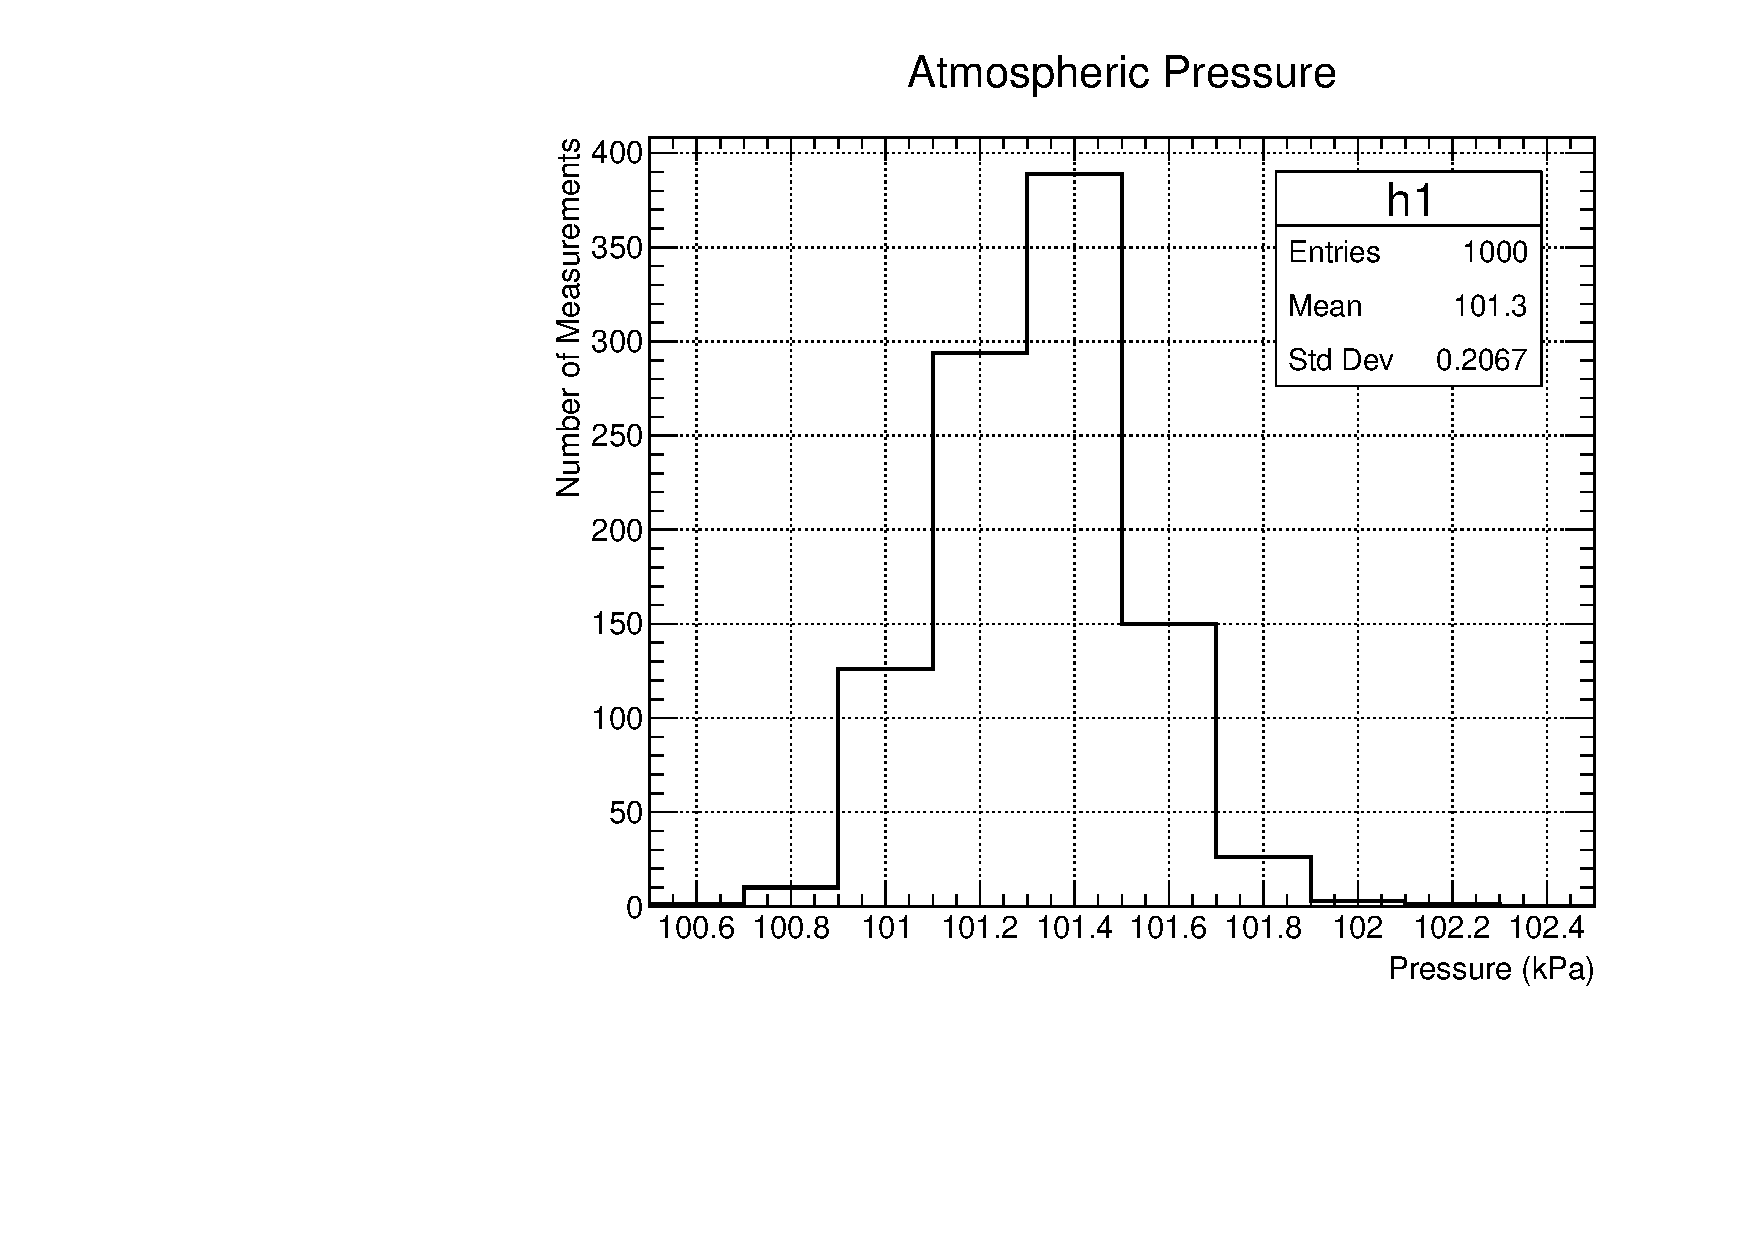
\includegraphics[angle=270,width=0.5\textwidth]{figures/histo.pdf}
\caption{\label{fig:histo} An example of a distribution of measurements from one instrument: a pressure gauge.}
\end{figure}

The true pressure is most likely 101.3 kPa.  The dial needle is moving, however, making identification of the true pressure impossible.  The true value is ascertained from the statistical distribution.  The \textit{mean} or average of the distribution is 101.3 kPa, and the \textit{standard deviation} is about 0.2 kPa.  Equation \ref{eq:std} represents the standard deviation procedure.  First, the mean $\bar{x}$ is calculated for the collection of measurements $x_i$.  Next, the quantity $(x_i - \bar{x})^2$ is computed for each $x_i$.  Next, the sum of these quantities is found, dividing by $N$\footnote{Technically, we should divide by $N-1$ since the mean has already accounted for one degree of freedom, but in practice where $N$ is a large number, this rarely matters.}, where $N$ is the number of measurements.  This result is called the \textit{variance}, $\sigma^2$.  Finally the square root of the variance is taken to find the standard deviation: $\sqrt{\sigma^2} = \sigma$.

\begin{equation}
\sigma_x = \sqrt{\frac{1}{N} \left( \sum_{i=1}^N (x_i - \bar{x})^2\right)} \label{eq:std}
\end{equation}

\section{Analysis of Data Subject to Random Error}

Imagine we are trying to measure the current flowing through a resistor by measuring the voltage across it, and measuring the resistance of the resistor.  The numbers should satisfy Ohm's law:

\begin{equation}
V = IR
\end{equation}

Suppose we make a measurement of the current, with an associated error: $I\pm \sigma_I$.  Now, we double the voltage, and measure the current (which should double).  What happens to the error $\sigma_I$?  Naturally, it should also double:

\begin{equation}
2(I\pm \sigma_I) = 2I \pm 2\sigma_I
\end{equation}

In general, for a variable $x$ being measured, multiplied by an error-less constant, we have

\begin{equation}
k(x\pm \sigma_x) = kx \pm k\sigma_x
\end{equation}

It turns out there are several rules for how to address the combination of variables subject to statistical error.  This is also called the \textit{propagation of errors.}

\subsection{Addition and Subtraction of variables with errors}

Suppose we are measuring the total resistance by measuring two resistors \textit{in series} individually, and summing them.  The resistances add, so

\begin{equation}
R_{tot} = R_1 + R_2
\end{equation}

Regarding addition and subtraction of variables $x\pm \sigma_x$ and $y\pm \sigma_y$, it turns out that

\begin{align}
(x\pm \sigma_x) + (y\pm \sigma_y) &= (x+y) \pm \sqrt{\sigma_x^2 + \sigma_y^2} \label{eq:add} \\
(x\pm \sigma_x) - (y\pm \sigma_y) &= (x-y) \pm \sqrt{\sigma_x^2 + \sigma_y^2}
\end{align}

Thus, the appropriate formula for our addition of resistances would be Eq. \ref{eq:add}:

\begin{equation}
(R_{1} \pm \sigma_{R1}) + (R_{2} \pm \sigma_{R2}) = (R_{1}+R_{2}) \pm \sqrt{\sigma_{R1}^2 + \sigma_{R2}^2}
\end{equation}

The pattern in Eq. \ref{eq:add} is called \textit{adding in quadrature}.  The formula for the error of added or subtracted variables $x$ and $y$ is

\begin{equation}
\sigma_{x\pm y} = \sqrt{\sigma_x^2 + \sigma_y^2}
\end{equation}

\subsection{Multiplication and Division of variables with errors}

Suppose we are trying to quantify the momentum of a system with mass $m$ and speed $v$:

\begin{equation}
p = mv
\end{equation}

We measure the mass: $m\pm \sigma_m$, and the speed: $v\pm\sigma_v$.  The \textit{fractional error} in the momentum, speed, and mass are $\frac{\sigma_p}{p}$, $\frac{\sigma_v}{v}$, and $\frac{\sigma_m}{m}$ respectively.  The relationship between the fractional error in momentum and the other two is

\begin{equation}
\left(\frac{\sigma_p}{p}\right)^2 = \left(\frac{\sigma_m}{m}\right)^2 + \left(\frac{\sigma_v}{v}\right)^2
\end{equation}

Notice that the fractional errors of the mass and speed are added in quadrature (summing squares) to produce the frational error of the momentum.  Thus, to quote a measurement of momentum, the result is:

\begin{equation}
p = (mv) \pm (mv) \sqrt{\left(\frac{\sigma_m}{m}\right)^2 + \left(\frac{\sigma_v}{v}\right)^2}
\end{equation}

In other words, when two variables are \textit{multiplied or divided}, the \textit{fractional errors} are combined rather than the \textit{absolute errors} as with variables that are \textit{added or subtracted.} In general, if $f=xy$ or $f = x/y$ or $f=y/x$:

\begin{equation}
\left(\frac{\sigma_f}{f}\right)^2 = \left(\frac{\sigma_x}{x}\right)^2 + \left(\frac{\sigma_y}{y}\right)^2 \label{eq:multi}
\end{equation}

\subsection{The General Case}

Suppose a function $f(x_1,x_2,x_3,...)$ combines the set of variables $x_i$ each subject to statistical error.  The \textit{variance} $\sigma_f^2$ is

\begin{equation}
\sigma_f^2 = \sum_i \sigma_{x_i}^2 \left( \frac{\partial f}{\partial x_i} \right)^2
\end{equation}

\textbf{For $f(x,y) = x+y$ and $g(x,y) = xy$, prove Eqs. \ref{eq:add} and \ref{eq:multi} below:} \\ \vspace{3cm}

\section{DC Circuit Lab}

Consider the \textbf{voltage divider} in Fig. \ref{fig:vd} (left).  We can show that the ratio of $V_{out}$ to $V_{in}$ is

\begin{equation}
\frac{V_{out}}{V_{in}} = \frac{R_2}{R_1+R_2}
\end{equation}

If the two resistors are equal the voltage is reduced by a factor of two, for example.  Consider the voltage divider in Fig. \ref{fig:vd} (right), with 4 ports.  We can select a voltage that is equal to the input voltage times one of four possible values.

\begin{figure}[hb]
\centering
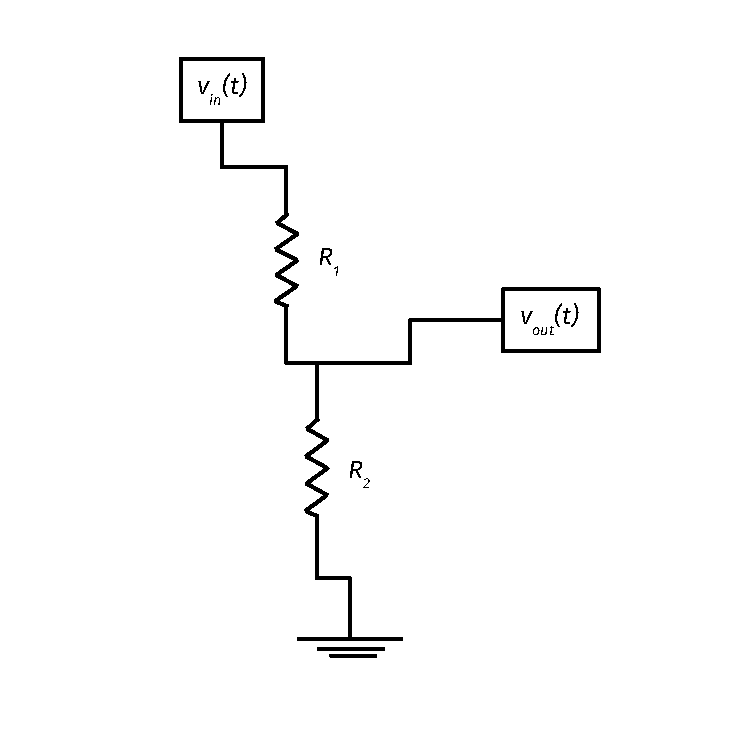
\includegraphics[width=0.4\textwidth]{figures/VoltageDivider.pdf}
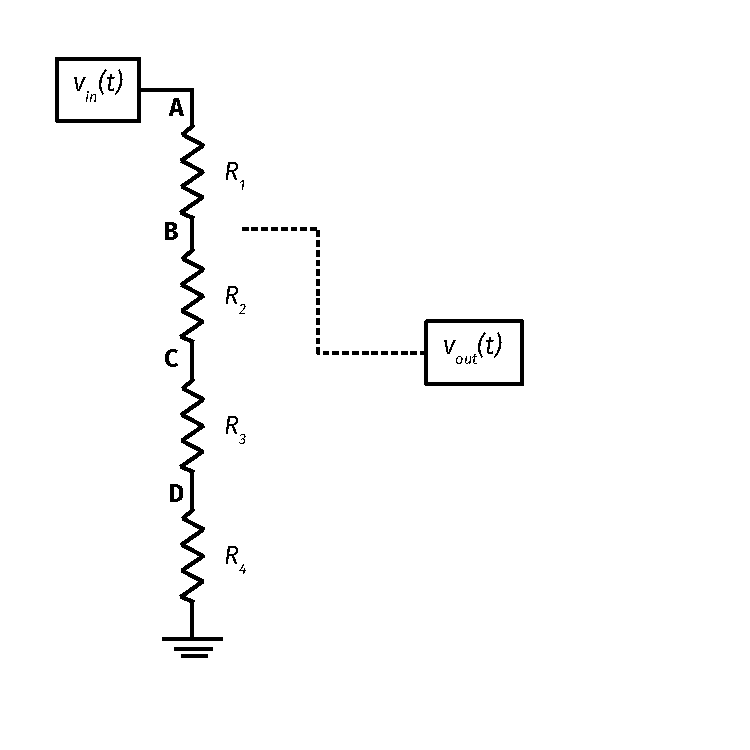
\includegraphics[width=0.4\textwidth]{figures/VoltageDivider2.pdf}
\caption{\label{fig:vd} (Left) This DC circuit is known as a voltage divider, because it can change a voltage by a fixed ratio. (Right) By connecting the output at different points, the ratio can be tuned.}
\end{figure}

\textbf{Procedure:}

\begin{enumerate}
\item Using the (1) breadboard, (2) DC power supply, (3) cables, (4) resistors, and (4) voltmeter, construct Fig. \ref{fig:vd} (right).
\item Place a voltage $\approx 4.0$ V as the input voltage, and use all four resistors in the voltage divider.
\item Record the voltage at the four locations \textbf{A through D.}  Associate a statistical error with each of your measurements.  Using the voltmeter, this is like assigning 100\% fractional error to the significant digit beyond the precision of the meter.  For example, if the meter reads 4.01, the error is 0.005 V.
\item Measure the resistances of $R_1$ through $R_4$, and record associated errors.
\item \textit{Predict the values of $V_{out}/V_{in}$} given the resistor values, including error propagation.
\item Do the measurements of $V_{out}/V_{in}$ agree with the predictions from the resistor values?  Why or why not?
\end{enumerate}

\end{document}